\newpage
\section{Aufgabe2}
\label{sec:a2}



\subsection{a)}
\label{subsec:a2a}

Siehe Python-Datei.

\subsection{b)}
\label{subsec:a2b}

\FloatBarrier
\begin{figure}
  \centering
  \includegraphics[width=\textwidth]{plot1.pdf}
  \caption{Histogramm bei Startwert 4000.}
  \label{fig:a2p1}
\end{figure}
\FloatBarrier

\FloatBarrier
\begin{figure}
  \centering
  \includegraphics[width=\textwidth]{plot2.pdf}
  \caption{Histogramm bei Startwert 15.}
  \label{fig:a2p2}
\end{figure}
\FloatBarrier

\FloatBarrier
\begin{figure}
  \centering
  \includegraphics[width=\textwidth]{plot3.pdf}
  \caption{Histogramm bei Startwert -4.}
  \label{fig:a2p3}
\end{figure}
\FloatBarrier
Anhand der Abbildungen \ref{fig:a2p1}, \ref{fig:a2p2} und \ref{fig:a2p3} lässt sich erkennen,
dass der Liniar-kongruente Generator die Anforderungen erfüllt . Dies ist der Fall da die erzeugten Werte zwischen $0$ und $1$ liegen und alle bins ungefähr gleich viele Treffer haben.
Dabei ist es unabhängig vom Start Wert ob eine Gleichverteilung dieser Art entsteht. Allerdings verschiebt eine andere Wahl des Startwerts die Struktur des Histogramms senkrecht zur
Richtung der Bin-Längen.

\subsection{c)}
\label{subsec:a2c}

\FloatBarrier
\begin{figure}
  \centering
  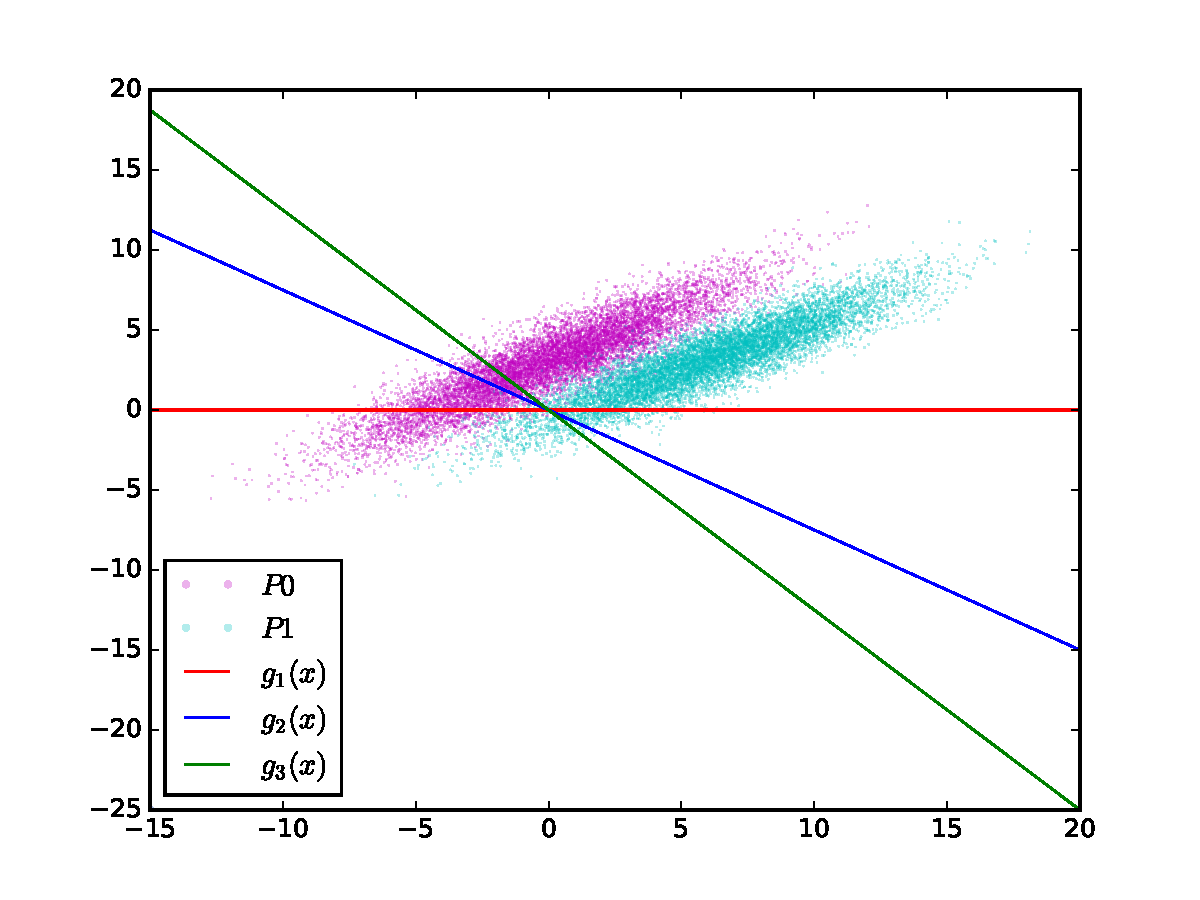
\includegraphics[width=\textwidth]{scatterplot2D.pdf}
  \caption{2D Streudiagramm.}
  \label{fig:a2p4}
\end{figure}
\FloatBarrier

\FloatBarrier
\begin{figure}
  \centering
  \includegraphics[width=\textwidth]{scatterplot3D.pdf}
  \caption{3D Streudiagramm.}
  \label{fig:a2p5}
\end{figure}
\FloatBarrier
Nein das Ergebnis entpricht nicht dem eines guten Zufallsgenerator, denn es ergeben sich im 2D wie 3D Plot eindeutig
erkennbare Muster . Dies deutet darauf hin, dass auf einander folgende Zahlen von einander abhängen.

\subsection{d)}
\label{subsec:a2d}


\subsection{e)}
\label{subsec:a2e}
